\section{Workload characterisation and metrics}
\begin{figure}[h]
  \centering
  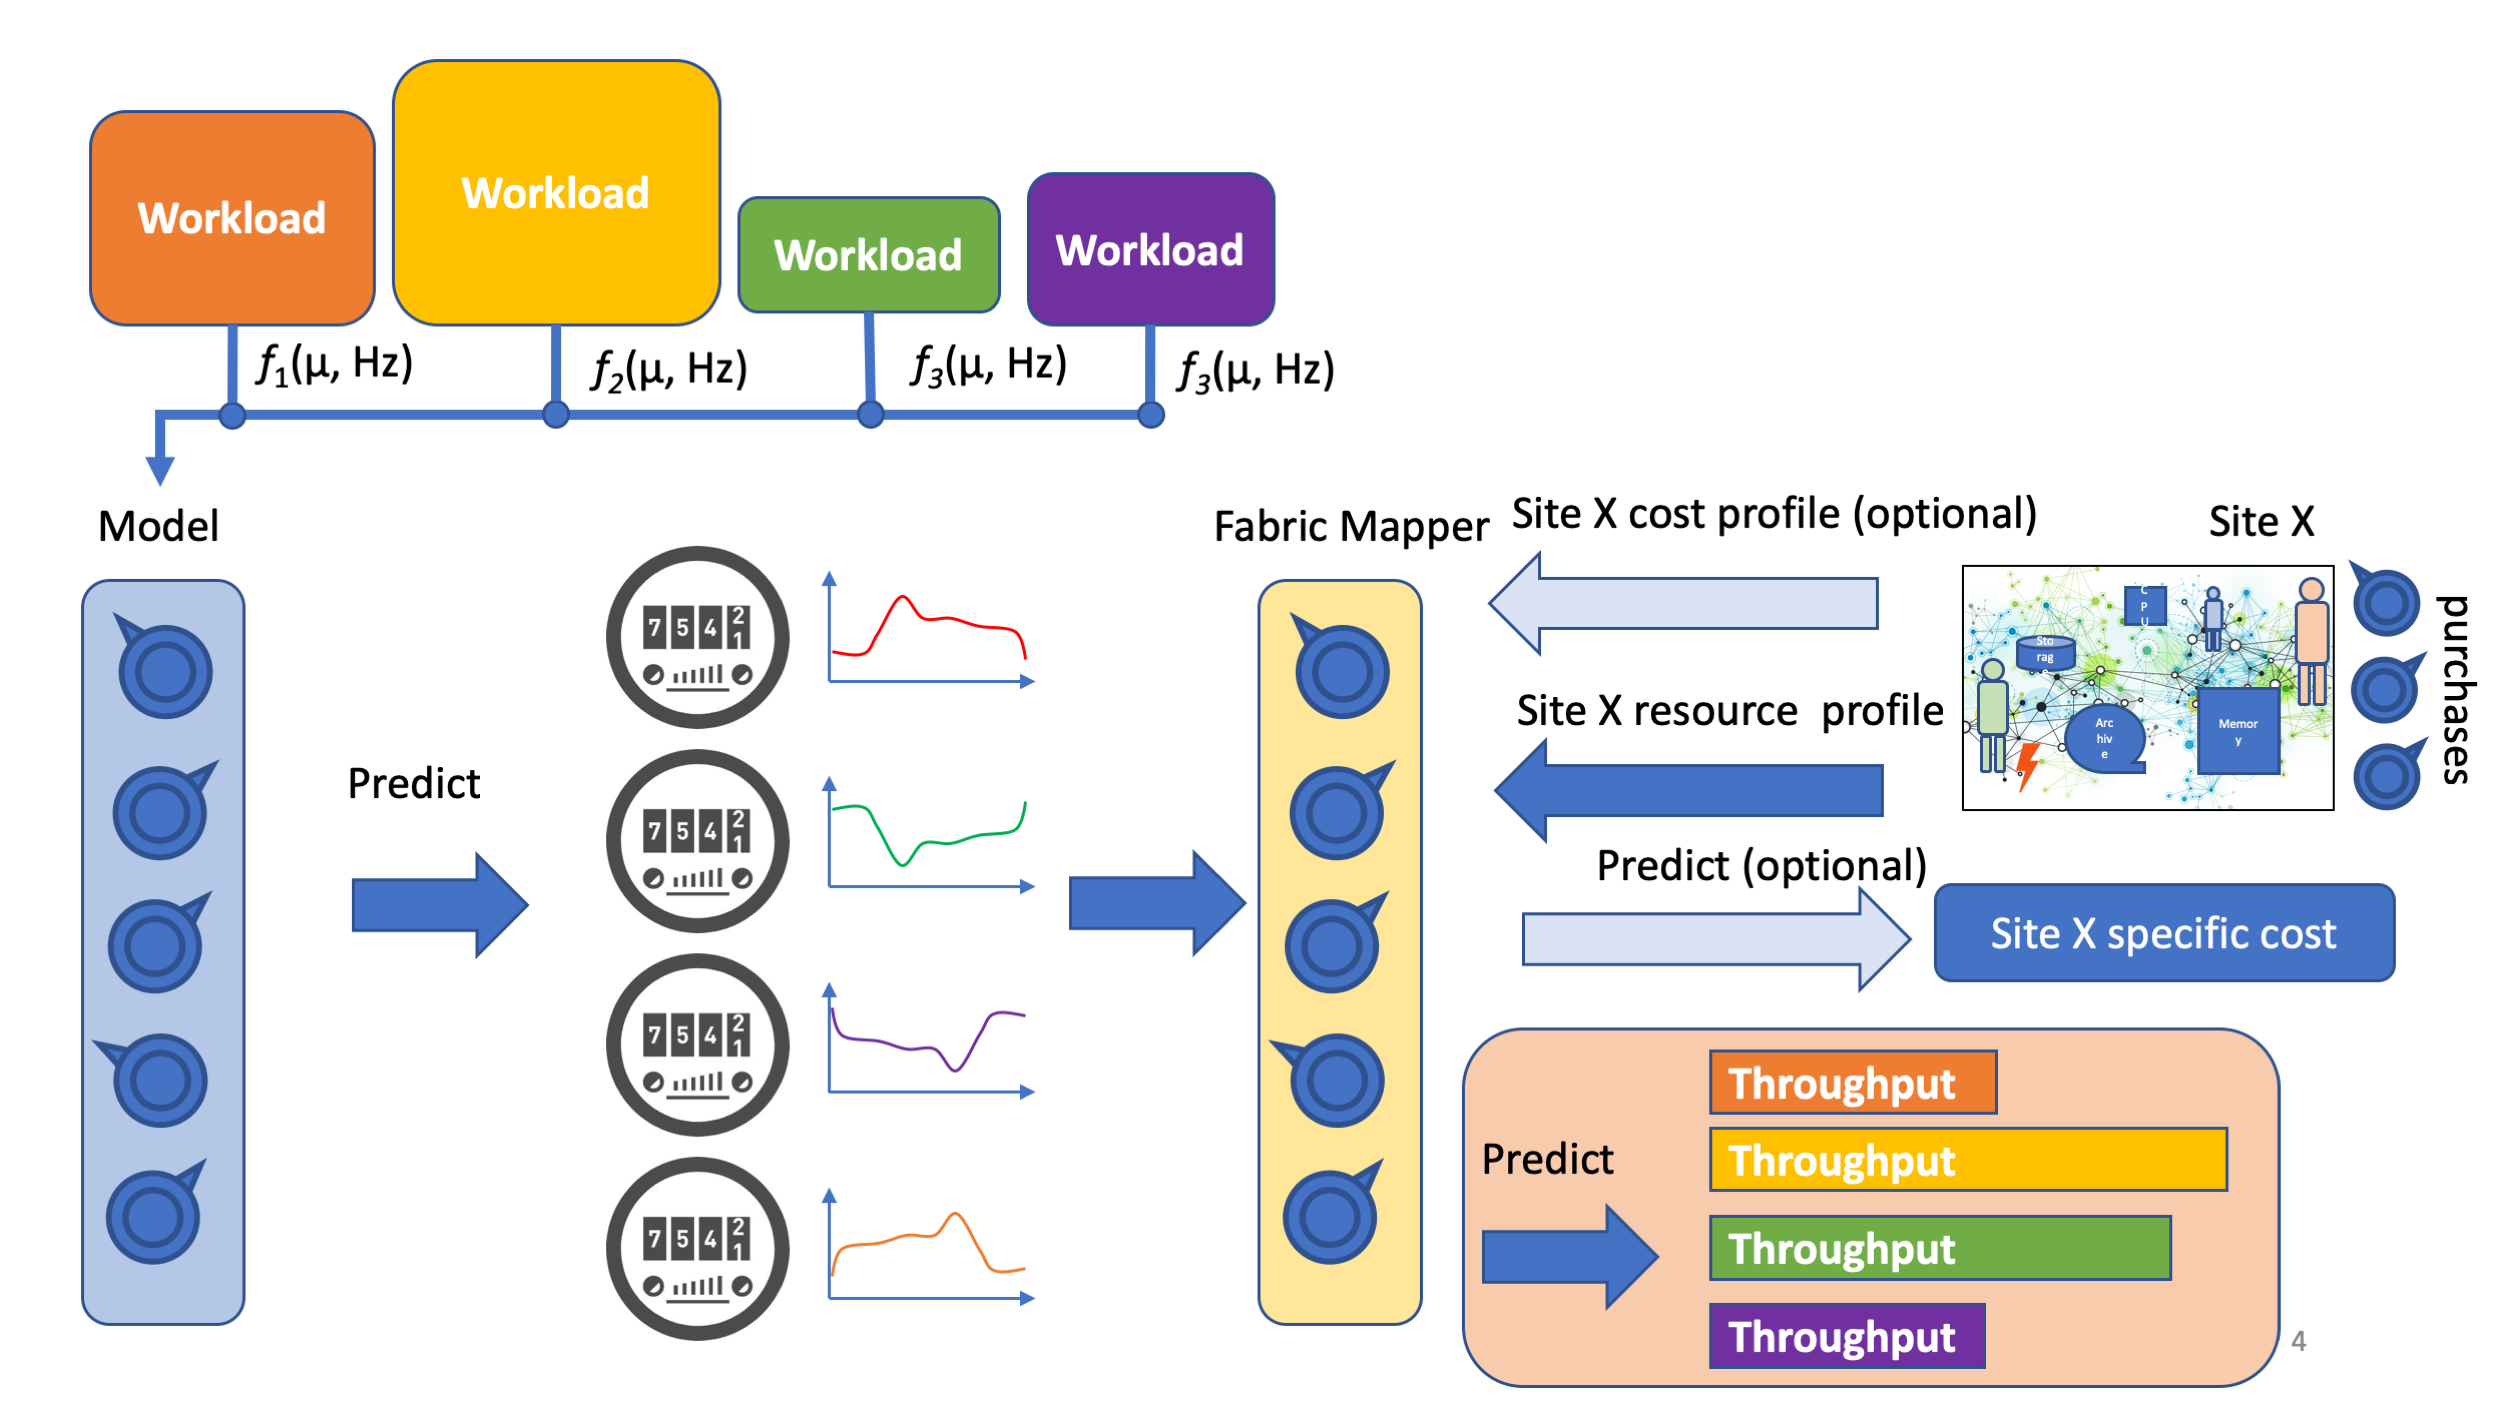
\includegraphics[height=4cm]{CHEP-Model-2.png}
  \hfill
  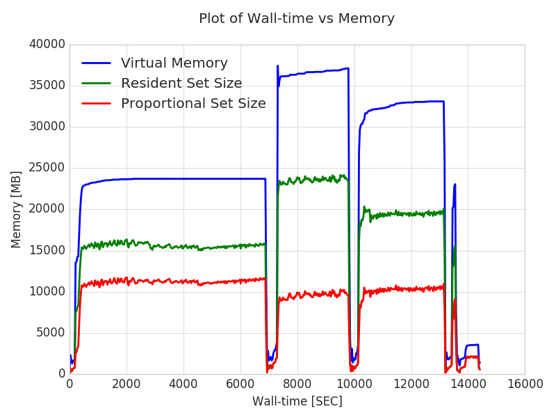
\includegraphics[height=4cm]{prmon.png}
  \caption{{\em (left)} Workload resource requirements depend on the
    pileup and the trigger rate. The model predicts the demands on the
    different resources. The Fabric Mapper abstracts the
    characteristics of a fabric and produces estimates for
    throughputs. Optional sites can add their local cost structure to
    the model. {\em (right)} Memory consumption over the execution of
    an ATLAS Digi-Reco job from PrMon; the different processing steps
    are clearly visible. The periods with very low memory consumption
    are due to the merging of intermediate files}
  \label{fig:mapping}
\end{figure}

To model the behaviour of the workloads of the LHC experiments it is
essential to understand how the different capabilities that a site
provides impact their throughput. To limit the complexity of a
performance model, it is desirable to minimise the number of
performance characteristics; this requires to find a set of
``orthogonal'' metrics to which the throughput is sensitive. This
knowledge can then be used by software developers to avoid bottlenecks
by balancing resource usage, and by site managers to optimise their
expenditure. The balance between the amount of memory per core, the
disk performance and the memory speed and latency can be optimised on
the basis of the characterisation of the relevant
workloads. Figure~\ref{fig:mapping} illustrates this relationship.

Finding such a metric set if far from trivial, given the complexity of
workloads and their production environments. We started from a
representative collection of reference workloads for each experiment.
Then, we listed several metrics, grouped in various categories (CPU,
I/O, memory, storage, swap and network) and assessed their
relevance. Finally we focused on those that can be measured without
significant interference with the running workload on nodes. A tool,
PrMon \cite{prmon}, originally developed by ATLAS, has been
generalised and allows to measure a large set of parameters, using
information from the operating system. Figure~\ref{fig:mapping} shows,
as an example, measurements of the memory usage during the execution
of a workload that performs digitisation with pile-up data and
reconstruction for Monte Carlo events.  PrMon allows to estimate which
capabilities of a system limit the throughput and how efficiently
multi-process and multi-threaded applications use their allocated
cores. To study the dependencies on latency, bandwidth and memory
restrictions, another tool has been developed that runs workloads
repeatedly with increasingly restricted bandwidth, memory and
increased latency, measuring the throughput for each configuration.

Another tool, Trident~\cite{trident}, was developed to provide a
convenient access to the information contained in CPU hardware
counters.  These counters provide information on the level of
parallelism exploited by a workload, memory access, cache utilisation
and vector capabilities, etc.~in an abstract and CPU-model dependent
way.  This gives the developer an estimate on how much improvement is
at best possible in exploiting the available resources and
quantitatively understand the limiting factors. The site managers can
use the insights gained from Trident in decisions concerning
trade-offs between different capabilities, like memory speed vs. size
or system disk speed and network.

\subsection{Next steps}
While the time series measured by PrMon give valuable insights, they
cannot be directly used as input for modelling the behaviour of the
workloads. Work on this process has started to parametrise metric time
series, as processing can be described as sequence of steps, each one
looping over events. During each of these steps the resource usage can
be described by a small number of parameters and the number of
processed events. This, in combination with the dependencies on
latency, bandwidth and memory, will allow to predict the throughput of
the current workloads under different conditions.

For the resource modelling under future running conditions the
dependency on the average pile-up has to integrated into the
model. For data size and simulation time, the dependency is at most
linear. For reconstruction, an extrapolation to HL-LHC levels is
currently very uncertain and it would be exponential with the current
algorithms. ATLAS plans to address this issue by introducing closely
spaced tracking layers, to provide precise starting vectors, while CMS
will take advantage of a very high time resolution to distinguish
between hits from different collisions.
